An einem Datum werden verschiedene Filme zu bestimmten Uhrzeiten gezeigt.
Jeder Film hat einen Titel und einen Regisseur.\\

\noindent
Erstellen Sie das Domänenmodell inklusive Attributen und Multiplizitäten.\\

\noindent
Welches Muster haben Sie wo und wie verwendet?


\section*{Antwort}
S. Abbildung~\ref{fig:film}.

\begin{figure}
    \centering
    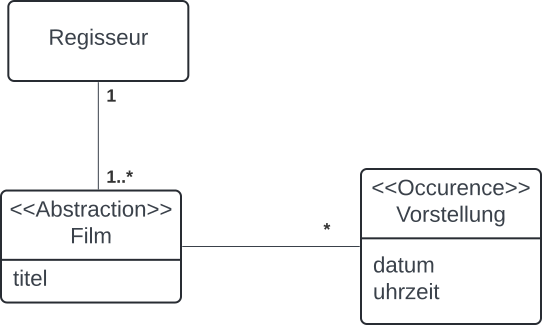
\includegraphics[scale=0.5]{chapters/aufgabe 3/img/film}
    \caption{Domänenmodell für Aufgabe 3. (Quelle: eigene)}
    \label{fig:film}
\end{figure}

\noindent
Anwendung des Musters \textbf{Exemplartyp} für die \code{Film}-\code{Vorstellung}-Assoziation.\\

\noindent
Hierdurch können redundate Informationen in Objekten des Typs \code{Film} vermieden werden: Mehrere Objekte vom Typ \code{Film} hätten sonst identische Attribute wie \code{datum} und \code{uhrzeit}.\\

\subsection*{Anmerkungen}
Ein Objekt vom Typ \code{Regisseur} wird in dem Modell als \textbf{Reference Object} verwendet: Ein Objekt vom Typ \code{Regisseur} hat in dem Entwurf eine eindeutige Identität, Objekte vom Typ \code{Film} sind mit diesen eindeutig assoziiert.\\
Die Assoziation \code{Regisseur} - \code{Film} wurde nicht als Exemplartyp angegeben, da \code{Regisseur} mit \code{Film} keine gemeinsamen Attribute teilt.
Aus diesem Grund kann \code{Film} nicht als Auftreten (\textit{Occurrence}) der Abstraktion von \code{Regissuer} verstanden werden.\\
Zwar kann ein Film als Werk des Regisseurs auch als Ausdruck seines künstlerischen Schaffens und damit im philosophischen Sinne auch als sein Auftreten verstanden werden: Bei den geg. Anforderungen ist es aber empfehlenswert, nur die Zugehörigkeitsbeziehung in dem Modell als solche zu abstrahieren.\\
Auch wenn also die Semantik in dem geg. Modell durch die Benamung der Klassen hervorgeht, wurde zur Verdeutlichung noch ein ein \textit{Assoziationsname} für die Beziehung \code{Regisseur} - \code{Film} (in dieser Leserichtung) angegeben.